\documentclass[10pt]{beamer}

\usetheme[progressbar=frametitle]{m}

\usepackage{booktabs}
\usepackage[scale=2]{ccicons}
\usepackage[T1]{fontenc} 
\usepackage[frenchb]{babel}

\usepackage{pgfplots}
%\usepackage{subfigure}
\usepackage[compatibility=false]{caption}
\usepackage{subcaption}
\usepgfplotslibrary{dateplot}

\title{Projet TM}
\subtitle{\huge Rain of Music}

\author{\Large \underline{Encadrants} : Jean-Michaël CELERIER\\
\hspace*{2.91cm}Myriam DESAINTE-CATHERINE \\
		\underline{Élèves} : Akané LEVY, Maxime PAILLASSA }

\institute{\centering 
		
\includegraphics[scale = 0.15]{logo}}
\date{}

\begin{document}

\maketitle

\begin{frame}
  \frametitle{Plan}
  \setbeamertemplate{section in toc}[sections numbered]
  \tableofcontents[hideallsubsections]
\end{frame}


\section{Objectifs du projet}

\begin{frame}
	\frametitle{Le projet global}
    \begin{itemize}
        \item Projet transverse avec l'option Robotique
        \item Collaboration avec les étudiants en Art de l'Université de Bilbao
        \item Réalisation d'une chorégraphie avec des robots quadrupèdes (Metabot) et des drones
        \item Les robots pourraient être équipés de haut-parleurs et de microphones 
    \end{itemize}
     \begin{figure}
     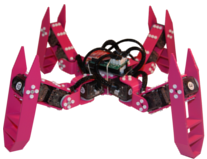
\includegraphics[scale=0.4]{metabot.png}
	\caption{Robot quadrupède utilisé : le Metabot}
    \end{figure}
\end{frame}

\begin{frame}
	\frametitle{Les différents participants du projet}
    \begin{itemize}
   		\item L'équipe de l'option Robotique s'occupera d'un système de localisation des robots et de communication entre eux
        \item Les étudiants de l'Université de Bilbao vont concevoir la chorégraphie
        \item Le LaBRI fournit le logiciel open source i-score pour l'écriture de la chorégraphie
	\end{itemize}
    
\begin{figure}[B]
\centering
\begin{subfigure}{.4\textwidth}
  \centering
  
\includegraphics[scale=0.5]{bilbao}
\end{subfigure}
\hspace*{1cm}
\begin{subfigure}{.4\textwidth}
  \centering
  
\includegraphics[scale=0.3]{labri}
\end{subfigure}
\end{figure}

\end{frame}


\begin{frame}
	\frametitle{Notre contribution}
    Réalisation d'un logiciel permettant la simulation et la visualisation de la chorégraphie écrite avec i-score.
    
 	Les problématiques : 
    \begin{itemize} 
    	\item La mise en place d'un environnement 3D (scène, caméra, objets)
        \item La communication avec i-score
        \item La simulation des mouvements des drones
        \item La détection de collision des robots
	\end{itemize}
   % Logiciel permettant aux artistes de simuler une chorégraphie. \\
   % Implique deux problématiques:
 

\end{frame}


\section{Outils de réalisation}

\begin{frame}
	\frametitle{Bibliothèques graphiques}
    \begin{itemize}
		\item OpenFrameworks : choix final, présente le plus de possibilités
        \item OpenSceneGraph : communauté peu active 
        \item OpenGL : productivité faible dûe à l'aspect bas niveau
        \item Unity : contrainte matérielle, non open source
        \item Babylon.js : JavaScript peu adapté à la taille du projet 
	\end{itemize}
    	\begin{figure}
     
\includegraphics[scale=0.15]{oflogo}
    \end{figure}
\end{frame}

\begin{frame}
	\frametitle{Protocole Minuit}
    \begin{itemize}
		\item Le logiciel i-score intègre le format de données Open Sound Control (OSC) via le protocole UDP
        \item Le protocole Minuit permet de structurer les données transmises avec OSC dans un arbre : 
        \begin{itemize}
   		\item Containers: un noeud qui contient la structure du sous-arbre
        \item Data: un noeud qui contient une valeur
	\end{itemize}
    	\end{itemize}

\end{frame}



\section{Avancement}
\begin{frame}
	\frametitle{État actuel du logiciel}
	\begin{figure}
     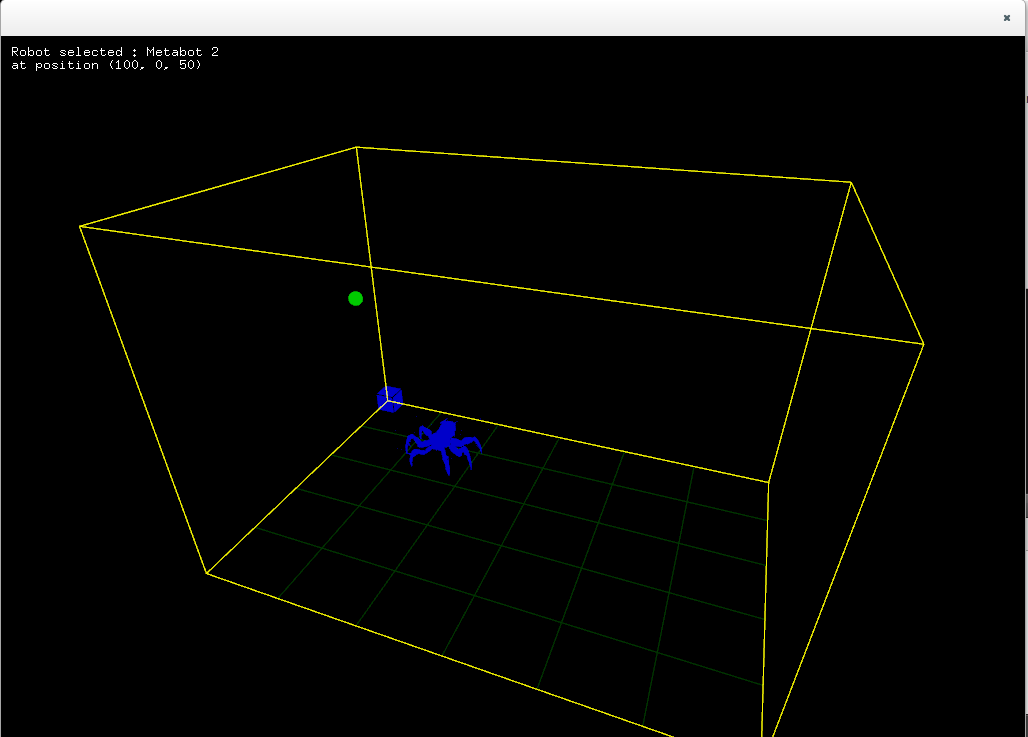
\includegraphics[scale=0.35]{screenshotRainofMusic.png}
	\caption{Capture d'écran du logiciel dans l'état actuel}
    \end{figure}
\end{frame}

\begin{frame}
	\frametitle{Diagramme de séquence (1/2)}
	\begin{figure}
     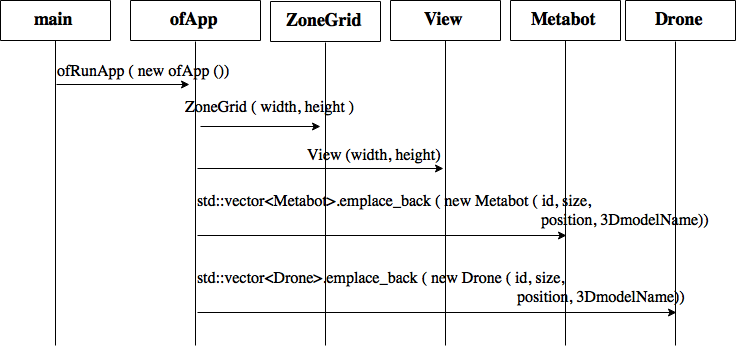
\includegraphics[scale=0.42]{diagramme_sequence_initialisation.png}
	\caption{Diagramme pour l'initialisation}
    \end{figure}
\end{frame}

\begin{frame}
	\frametitle{Diagramme de séquence (2/2)}
	\begin{figure}
     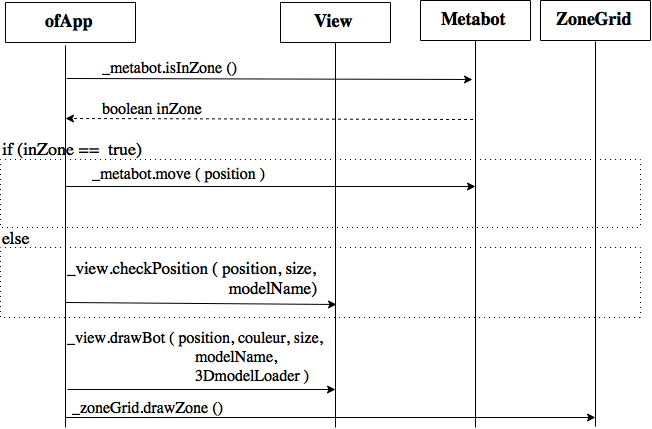
\includegraphics[scale=0.45]{diagramme_sequence_draw.png}
	\caption{Diagramme pour l'affichage}
    \end{figure}
\end{frame}



\begin{frame}
	\frametitle{Planning et organisation}
	\begin{figure}
     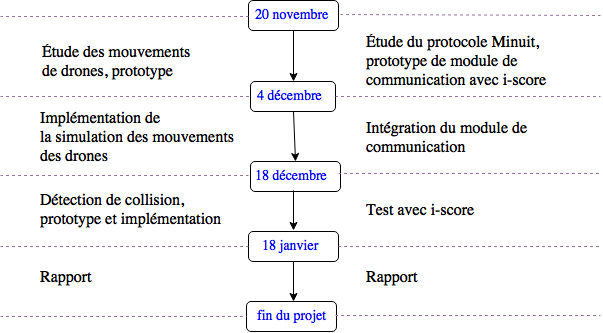
\includegraphics[scale=0.5]{calendrier.png}
	%\caption{Calendrier pour le projet}
    \end{figure}
\end{frame}

	\plain{Merci de votre attention. \\
    Des questions ?}

\end{document}
